\chapter{Mixed-frequency data}
\label{chap:mixed-frequency}

\section{Basics}
\label{sec:mixed-basics}

In some cases one may want to handle data that are observed at
different frequencies, a facility known as ``MIDAS'' (Mixed Data
Sampling). A common pairing includes GDP, usually available quarterly,
and industrial production, often available monthly. The most common
context when this feature is required is specification and estimation
of MIDAS models (see Chapter \ref{chap:MIDAS}), but other cases are
possible.

A gretl dataset formally handles only a single data frequency, but we
have adopted a straightforward means of representing nested
frequencies: a higher frequency series $x_H$ is represented by a set
of $m$ series, each holding the value of $x_H$ in a sub-period of the
``base'' (lower-frequency) period (where $m$ is the ratio of the
higher frequency to the lower).

This is most easily understood by means of an example. Suppose our
base frequency is quarterly and we wish to include a monthly series in
the analysis. Then a relevant fragment of the gretl dataset might look
as shown in Table~\ref{tab:mdata}. Here, \texttt{gdpc96} is a
quarterly series while \texttt{indpro} is monthly, so $m=12/4=3$ and
the per-month values of \texttt{indpro} are identified by the suffix
\verb|_m|\textit{n}, $n=3,2,1$.

\begin{table}[h]
\small
\begin{verbatim}
                   gdpc96    indpro_m3    indpro_m2    indpro_m1

      1947:1      1934.47      14.3650      14.2811      14.1973
      1947:2      1932.28      14.3091      14.3091      14.2532
      1947:3      1930.31      14.4209      14.3091      14.2253
      1947:4      1960.70      14.8121      14.7562      14.5606
      1948:1      1989.54      14.7563      14.9240      14.8960
      1948:2      2021.85      15.2313      15.0357      14.7842
\end{verbatim}
  \caption{A slice of MIDAS data}
  \label{tab:mdata}
\end{table}

To recover the actual monthly time series for \texttt{indpro} one must
read the three relevant series right-to-left by row. At first glance
this may seem perverse, but in fact it is the most convenient setup
for MIDAS analysis. In such models, the high-frequency variables are
represented by lists of lags, and of course in econometrics it is
standard to give the most recent lag first
$(x_{t-1}, x_{t-2}, \ldots)$.

One can construct such a dataset manually from ``raw'' sources using
hansl's matrix-handling methods or the \texttt{join} command (see
Section \ref{sec:data-methods} for illustrations), but we have added
native support for the common cases shown below.

\begin{center}
\begin{tabular}{ll}
\textit{base frequency} & \textit{higher frequency} \\[4pt]
annual    & quarterly or monthly \\
quarterly & monthly or daily \\
monthly   & daily
\end{tabular}
\end{center}

The examples below mostly pertain to the case of quarterly plus
monthly data. Section \ref{sec:midas-daily} has details on handling of
daily data.

A mixed-frequency dataset can be created in either of two ways: by
selective importation of series from a database, or by creating two
datasets of different frequencies then merging them.

\subsection{Importation from a database}
\label{sec:db-import}

Here's a simple example, in which we draw from the \texttt{fedstl} (St
Louis Fed) database which is supplied in the gretl distribution:
\begin{code}
clear
open fedstl.bin
data gdpc96
data indpro --compact=spread
store gdp_indpro.gdt
\end{code}

Since \texttt{gdpc96} is a quarterly series, its importation via the
\texttt{data} command establishes a quarterly dataset. Then the
MIDAS work is done by the option \verb|--compact=spread| for the
second invocation of \texttt{data}. This ``spreads'' the series
\texttt{indpro}---which is monthly at source---into three quarterly
series, exactly as shown in Table~\ref{tab:mdata}.

\subsection{Merging two datasets}
\label{sec:data-merge}

In this case we consider an Excel file provided by Eric Ghysels in his
\textsf{MIDAS Matlab Toolbox},\footnote{See
  \url{http://eghysels.web.unc.edu/} for links.} namely
\texttt{mydata.xlsx}.  This contains quarterly real GDP in Sheet1 and
monthly non-farm payroll employment in Sheet2. A hansl script to build
a MIDAS-style file named \texttt{gdp\_payroll\_midas.gdt} is shown in
Listing~\ref{lst:ghysels-data}.

\begin{script}[htbp]
  \caption{Building a gretl MIDAS dataset via merger}
  \label{lst:ghysels-data}
\begin{scode}
# sheet 2 contains monthly employment data
open MIDASv2.2/mydata.xlsx --sheet=2
rename VALUE payems
dataset compact 4 spread
# limit to the sample range of the GDP data
smpl 1947:1 2011:2
setinfo payems_m3 --description="Non-farm payroll employment, month 3 of quarter"
setinfo payems_m2 --description="Non-farm payroll employment, month 2 of quarter"
setinfo payems_m1 --description="Non-farm payroll employment, month 1 of quarter"
store payroll_midas.gdt

# sheet 1 contains quarterly GDP data
open MIDASv2.2/mydata.xlsx --sheet=1
rename VALUE qgdp
setinfo qgdp --description="Real quarterly US GDP"
append payroll_midas.gdt
store gdp_payroll_midas.gdt
\end{scode}
\end{script}

Note that both series are simply named \texttt{VALUE} in the source
file, so we use gretl's \texttt{rename} command to set distinct and
meaningful names. The heavy lifting is done here by the line
%
\begin{code}
dataset compact 4 spread
\end{code}
%
which tells gretl to compact an entire dataset (in this case, as it
happens, just containing one series) to quarterly frequency using the
``spread'' method. Once this is done, it is straightforward to
\texttt{append} the compacted data to the quarterly GDP dataset.

We will put an extended version of this dataset (supplied with gretl,
and named \texttt{gdp\_midas.gdt}) to use in subsequent sections.

\section{The notion of a ``MIDAS list''}
\label{sec:midas-list}

In the following two sections we'll describe functions that (rather
easily) do the right thing if you wish to create lists of lags or
first differences of high-frequency series. However, we should first
be clear about the correct domain for such functions, since they could
produce the most diabolical mash-up of your data if applied to the
wrong sort of list argument---for instance, a regular list containing
distinct series, all observed at the ``base frequency'' of the
dataset.

So let us define a \textbf{MIDAS list}: this is a list of $m$ series
holding per-period values of a \textit{single} high-frequency series,
arranged in the order of most recent first, as illustrated
above. Given the dataset shown in Table~\ref{tab:mdata}, an example
of a correctly formulated MIDAS list would be
%
\begin{code}
list INDPRO = indpro_m3 indpro_m2 indpro_m1
\end{code}
%
Or, since the monthly observations are already in the required order,
we could define the list by means of a ``wildcard'':
%
\begin{code}
list INDPRO = indpro_m*
\end{code}

Having created such a list, one can use the \texttt{setinfo} command
to tell gretl that it's a \textit{bona fide} MIDAS list:
%
\begin{code}
setinfo INDPRO --midas
\end{code}
%
This will spare you some warnings that gretl would otherwise emit when
you call some of the functions described below. This step should not
be necessary, however, if the series in question are the product of a
\texttt{compact} operation with the \texttt{spread} parameter.

\subsection{Inspecting high-frequency data}

The layout of high-frequency data shown in Table~\ref{tab:mdata} is
convenient for running regressions, but not very convenient for
inspecting and checking such data. We therefore provide some methods
for displaying MIDAS data at their ``natural''
frequency. Figure~\ref{fig:data-menu} shows the gretl main window with
the \texttt{gdp\_midas} dataset loaded, along with the menu that pops
up if you right-click with the \texttt{payems} series highlighted.
The items ``Display values'' and ``Time series plot'' show the data
on their original monthly calendar, while the ``Display components''
item shows the three component series on a quarterly calendar, as
in Table~\ref{tab:mdata}.

These methods are also available via the command line. For example,
the commands
%
\begin{code}
list PAYEMS = payems_*
print PAYEMS --byobs --midas
hfplot PAYEMS --with-lines --output=display
\end{code}
%
produce a monthly printout of the payroll employment data, followed by
a monthly time-series plot. (See section~\ref{sec:hfplot} for more on
\texttt{hfplot}.)

\begin{figure}[htbp]
  \centering
  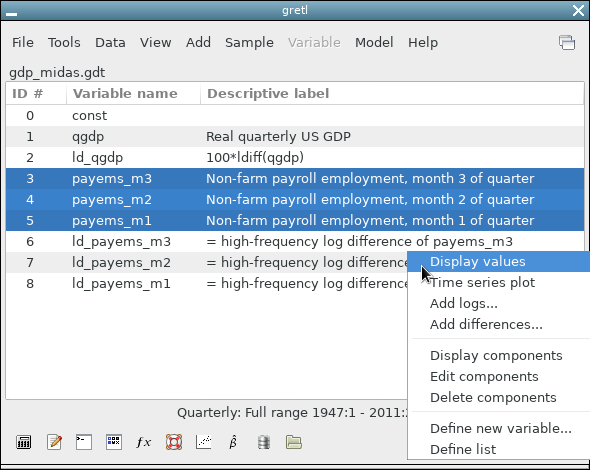
\includegraphics[scale=0.5]{figures/midas-list-menu}
  \caption{MIDAS data menu}
  \label{fig:data-menu}
\end{figure}


\section{High-frequency lag lists}
\label{sec:hflags}

A basic requirement of MIDAS is the creation of lists of
high-frequency lags for use on the right-hand side of a regression
specification. This is possible, but not very convenient, using the
gretl's \texttt{lags} function; it is made easier by a dedicated
variant of that function described below.

For illustration we'll consider an example presented in Ghysels'
\textsf{Matlab} implementation of MIDAS: this uses 9 monthly lags of
payroll employment, starting at lag 3, in a model for quarterly GDP.
The estimation period for this model starts in 1985Q1. At this
observation, the stipulation that we start at lag 3 means that the
first (most recent) lag is employment for October 1984,\footnote{That
  is what Ghysels means, but see the sub-section on ``Leads and
  nowcasting'' below for a possible ambiguity in this regard.} and the
9-lag window means that we need to include monthly lags back to
February 1984. Let the per-month employment series be called
\texttt{x\_m3}, \texttt{x\_m2} and \texttt{x\_m1}, and let (quarterly)
lags be represented by \texttt{(-1)}, \texttt{(-2)} and so on. Then
the terms we want are (reading left-to-right by row):
\begin{center}
{\small
\begin{tabular}{ccc}
 . & . & \texttt{x\_m1(-1)} \\
\texttt{x\_m3(-2)} & \texttt{x\_m2(-2)} & \texttt{x\_m1(-2)} \\
\texttt{x\_m3(-3)} & \texttt{x\_m2(-3)} & \texttt{x\_m1(-3)} \\
\texttt{x\_m3(-4)} & \texttt{x\_m2(-4)} & .
\end{tabular}
}
\end{center}

We could construct such a list in gretl using the following
standard syntax. (Note that the third argument of 1 to
\texttt{lags} below tells gretl that we want the terms ordered ``by
lag'' rather than ``by variable''; this is required to respect the
order of the terms shown above.)
\begin{code}
list X = x_m*
# create lags for 4 quarters, "by lag"
list XL = lags(4,X,1)
# convert the list to a matrix
matrix tmp = XL
# trim off the first two elements, and the last
tmp = tmp[3:11]
# and convert back to a list
XL = tmp
\end{code}

However, the following specialized syntax is more convenient:
\begin{code}
list X = x_m*
setinfo X --midas
# create high-frequency lags 3 to 11
list XL = hflags(3, 11, X)
\end{code}

In the case of \texttt{hflags} the length of the list given as the
third argument defines the ``compaction ratio'' ($m=3$ in this
example); we can (in fact, must) specify the lags we want in
high-frequency terms; and ordering of the generated series by lag is
automatic. 

Word to the wise: do not use \texttt{hflags} on anything other than a
\textbf{MIDAS list} as defined in section~\ref{sec:midas-list}, unless
perhaps you have some special project in mind and really know what you
are doing.

\subsection{Leads and nowcasting}

Before leaving the topic of lags, it is worth commenting on the
question of leads and so-called ``nowcasting''---that is, prediction
of the current value of a lower-frequency variable before its
measurement becomes available.

In a regular dataset where all series are of the same frequency,
lag 1 means the observation from the previous period, lag 0 is
equivalent to the current observation, and lag $-1$ (or lead 1) is the
observation for the next period into the relative future.

When considering high-frequency lags in the MIDAS context, however,
there is no uniquely determined high-frequency sub-period which is
temporally coincident with a given low-frequency period. The placement
of high-frequency lag 0 therefore has to be a matter of
convention. Unfortunately, there are two incompatible conventions in
currently available MIDAS software, as follows.
%
\begin{itemize}
\item High-frequency lag 0 corresponds to the \textit{first}
  sub-period within the current low-frequency period. This is what we
  find in Eric Ghysels' \textsf{MIDAS Matlab Toolbox}; it's also
  clearly stated and explained in \cite{armesto10}.
\item High-frequency lag 0 corresponds to the \textit{last} sub-period
  in the current low-frequency period. This convention is employed in
  the \texttt{midasr} package for \textsf{R}.\footnote{See
    \url{http://cran.r-project.org/web/packages/midasr/}, and for
    documentation
    \url{https://github.com/mpiktas/midasr-user-guide/raw/master/midasr-user-guide.pdf}.}
\end{itemize}
%
Consider, for example, the quarterly/monthly case. In \textsf{Matlab},
high-frequency (HF) lag 0 is the first month of the current quarter,
HF lag 1 is the last month of the prior quarter, and so on. In
\texttt{midasr}, however, HF lag 0 is the last month of the current
quarter, HF lag 1 the middle month of the quarter, and HF lag 3
is the first one to take you ``back in time'' relative to the start
of the current quarter, namely to the last month of the prior
quarter.

In gretl we have chosen to employ the first of these
conventions. So lag 1 points to the most recent sub-period in the
previous base-frequency period, lag 0 points to the first sub-period
in the current period, and lag $-1$ to the second sub-period within
the current period. Continuing with the quarterly/monthly case,
monthly observations for lags 0 and $-1$ are likely to become
available before a measurement for the quarterly variable is published
(possibly also a monthly value for lag $-2$). The first ``truly
future'' lead does not occur until lag $-3$.

The \texttt{hflags} function supports negative lags. Suppose one
wanted to use 9 lags of a high-frequency variable,
$-1, 0, 1,\ldots, 7$, for nowcasting. Given a suitable MIDAS list,
\texttt{X}, the following would do the job:
\begin{code}
list XLnow = hflags(-1, 7, X)
\end{code}

This means that one could generate a forecast for the current
low-frequency period (which is not yet completed and for which no
observation is available) using data from two sub-periods into the
low-frequency period (e.g.\ the first two months of the quarter).

\section{High-frequency first differences}

When working with non-stationary data one may wish to take first
differences, and in the MIDAS context that probably means
high-frequency differences of the high-frequency data. Note that the
ordinary gretl functions \texttt{diff} and \texttt{ldiff} will
\textit{not} do what is wanted for series such as \texttt{indpro}, as
shown in Table~\ref{tab:mdata}: these functions will give per-month
\textit{quarterly} differences of the data (month 3 of the current
quarter minus month 3 of the previous quarter, and so on).

To get the desired result one could create the differences before
compacting the high-frequency data but this may not be convenient, and
it's not compatible with the method of constructing a MIDAS dataset
shown in section~\ref{sec:db-import}. The alternative is to employ the
specialized differencing function \texttt{hfdiff}. This takes one
required argument, a \textbf{MIDAS list} as defined in
section~\ref{sec:midas-list}. A second, optional argument is a scalar
multiplier (with default value 1.0); this permits scaling the output
series by a constant. There's also an \texttt{hfldiff} function for
creating high-frequency log differences; this has the same syntax as
\texttt{hfdiff}.

So for example, the following creates a list of high-frequency
percentage changes (100 times log-difference) then a list of
high-frequency lags of the changes.
%
\begin{code}
list X = indpro_*
setinfo X --midas
list dX = hfldiff(X, 100)
list dXL = hflags(3, 11, dX)
\end{code}

If you only need the series in the list \texttt{dXL}, however, you can
nest these two function calls:
%
\begin{code}
list dXL = hflags(3, 11, hfldiff(X, 100))
\end{code}


\section{MIDAS-related plots}
\label{sec:hfplot}

In the context of MIDAS analysis one may wish to produce time-series
plots which show high- and low-frequency data in correct registration
(as in Figures 1 and 2 in \citealp{armesto10}).  This can be done using
the \texttt{hfplot} command, which has the following syntax:

\texttt{hfplot} \textsl{midas-list} \texttt{[; }\textsl{lflist} 
\texttt{]} \textsl{options}

The required argument is a MIDAS list, as defined above. Optionally,
one or more lower-frequency series (\textsl{lflist}) can be added to
the plot following a semicolon. Supported options are
\option{with-lines}, \option{time-series} and \option{output}. These
have the same effects as with the gretl's \texttt{gnuplot} command.

An example based on Figure 1 in \cite{armesto10} is shown in
Listing~\ref{ex:midas-armesto} and Figure~\ref{fig:armesto}.

\begin{script}[p]
  \scriptinfo{midas-armesto}{Replication of a plot from Armesto et al}
\begin{scode}
open gdp_midas.gdt

# form and label the dependent variable
series dy = log(qgdp/qgdp(-1))*400
setinfo dy --graph-name="GDP"

# form list of annualized HF differences
list X = payems*
list dX = hfldiff(X, 1200)
setinfo dX --graph-name="Payroll Employment"

smpl 1980:1 2009:1
hfplot dX ; dy --with-lines --time-series --output=display
\end{scode}
\end{script}

\begin{figure}[p]
  \centering
  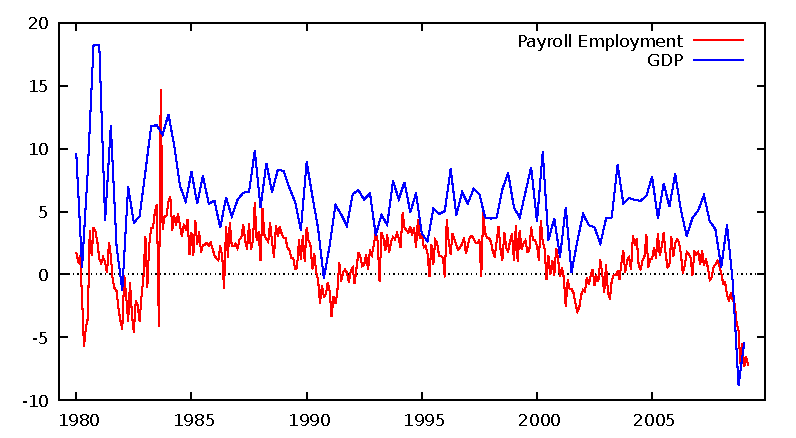
\includegraphics{figures/armesto_plot}
  \caption{Quarterly GDP and monthly Payroll Employment,
  annualized percentage changes}
  \label{fig:armesto}
\end{figure}

\section{Alternative MIDAS data methods}
\label{sec:data-methods}

\subsection*{Importation via a column vector}

Listing~\ref{ex:midas-list} illustrates how one can construct via hansl a
MIDAS list from a matrix (column vector) holding data of a higher
frequency than the given dataset. In practice one would probably read
high frequency data from file using the \texttt{mread} function, but
here we just construct an artificial sequential vector.

Note the check in the \texttt{high\_freq\_list} function: we determine
the current sample size, \texttt{T}, and insist that the input matrix
is suitably dimensioned, with a single column of length equal to
\texttt{T} times the compaction factor (here 3, for monthly to
quarterly).

\begin{script}[htbp]
  \scriptinfo{midas-list}{Create a midas list from a matrix}
\begin{scode}
function list high_freq_list (const matrix x, int compfac, string vname)
  list ret = deflist()
  scalar T = $nobs
  if rows(x) != compfac*T || cols(x) != 1
     funcerr "Invalid x matrix"
  endif
  matrix m = mreverse(mshape(x, compfac, T))'
  loop i=1..compfac
    scalar k = compfac + 1 - i
    ret += genseries(sprintf("%s%d", vname, k), m[,i])
  endloop
  setinfo ret --midas 
  return ret
end function

# construct a little "quarterly" dataset
nulldata 12
setobs 4 1980:1

# generate "monthly" data, 1,2,...,36
matrix x = seq(1,3*$nobs)'
print x
# turn into midas list
list H = high_freq_list(x, 3, "test_m")
print H --byobs
\end{scode}
\end{script}

The final command in the script should produce

{
\small
\begin{verbatim}
            test_m3      test_m2      test_m1

1980:1            3            2            1
1980:2            6            5            4
1980:3            9            8            7
...
\end{verbatim}
}

This functionality is available in the built-in function
\texttt{hflist}, which has the same signature as the hansl prototype
above.

\subsection*{Importation via \texttt{join}}

The \texttt{join} command provides a general and flexible framework
for importing data from external files (see chapter \ref{chap:join}). 

In order to handle multiple-frequency data, it supports the
``spreading'' of high-frequency series to a MIDAS list in a single
operation. This requires use of the \verb|--aggr| option with
parameter \texttt{spread}. There are two acceptable forms of usage,
illustrated below. Note that \texttt{AWM} is a quarterly dataset while
\texttt{hamilton} is monthly. First case:
%
\begin{code}
open AWM.gdt
join hamilton.gdt PC6IT --aggr=spread
\end{code}
and second case:
\begin{code}
open AWM.gdt
join hamilton.gdt PCI --data=PC6IT --aggr=spread
\end{code}

In the first case MIDAS series \texttt{PC6IT\_m3}, \texttt{PC6IT\_m2}
and \texttt{PC6IT\_m1} are added to the working dataset. In the second
case ``\texttt{PCI}'' is used as the base name for the imports,
giving \texttt{PCI\_m3}, \texttt{PCI\_m2} and \texttt{PCI\_m1}
as the names of the per-month series.

Note that only one high-frequency series can be imported in a given
\texttt{join} invocation with the option \verb|--aggr=spread|, which
already implies the writing of multiple series in the lower frequency
dataset.

An important point to note is that the \verb|--aggr=spread| mechanism
(where we map from one higher-frequency series to a set of
lower-frequency ones) relies on finding a known, reliable time-series
structure in the ``outer'' data file. Native gretl time-series data
files will have such a structure, and also well-formed gretl-friendly
CSV files, but not arbitrary comma-separated files.  So if you have
difficulty importing data MIDAS-style from a given CSV file using
\verb|--aggr=spread| you might want to drop back to a more agnostic,
piece-wise approach (agnostic in the sense of assuming less about
gretl's ability to detect any time-series structure that might be
present). Here's an example:
%
\begin{code}
open hamilton.gdt
# create month-of-quarter series for filtering
series mofq = ($obsminor - 1) % 3 + 1
# write example CSV file: the first column holds, e.g. "1973M01"
store test.csv PC6IT mofq
open AWM.gdt -q
# import monthly components one at a time, using a filter
join test.csv PCI_m3 --data=PC6IT --tkey=",%YM%m" --filter="mofq==3"
join test.csv PCI_m2 --data=PC6IT --tkey=",%YM%m" --filter="mofq==2"
join test.csv PCI_m1 --data=PC6IT --tkey=",%YM%m" --filter="mofq==1"
list PCI = PCI_*
setinfo PCI --midas
print PCI_m* --byobs
\end{code}
%$

The example is artificial in that a time-series CSV file of suitable
frequency written by gretl itself should work without special
treatment. But you may have to add ``helper'' columns (such as the
\texttt{mofq} series above) to a third-party CSV file to enable a
piece-wise MIDAS join via filtering.

% \clearpage

\subsection{Daily data}
\label{sec:midas-daily}

Daily data (commonly financial-market data) are often used in practical
applications of the MIDAS methodology. It's therefore important that
gretl support use of such data, but there are special issues arising
from the fact that the number of days in a month, quarter or year is
not a constant.

It seems to us that it's necessary to stipulate a fixed, conventional
number of days per lower-frequency period (that is, in practice, per
month or quarter, since for the moment we're ignoring the week as a
basic temporal unit and we're not yet attempting to support the
combination of annual and daily data). But matters are further
complicated by the fact that daily data come in (at least) three
sorts: 5 days per week (as in financial-market data), 6-day (some
commercial data which skip Sunday) and 7-day.

That said, we currently support---via \texttt{compact=spread}, as
described in section~\ref{sec:mixed-basics}---the following
conversions:
\begin{itemize}
\item Daily to monthly: If the daily data are 5-days per week, we
  impose 22 days per month. This is the median, and also the mode, of
  weekdays per month, although some months have as few as 20 weekdays
  and some have 23. If the daily data are 6-day we impose
  26 days per month, and in the 7-day case, 30 days per month.

\item Daily to quarterly: In this case the stipulated days per quarter
  are simply 3 times the days-per-month values specified above.
\end{itemize}

So, given a daily dataset, you can say
%
\begin{code}
dataset compact 12 spread
\end{code}
%
to convert MIDAS-wise to monthly (or substitute \texttt{4} for
\texttt{12} for a quarterly target). And this is supposed to work
whether the number of days per week is 5, 6 or 7.

That leaves the question of how we handle cases where the actual
number of days in the calendar month or quarter falls short of, or
exceeds, the stipulated number. We'll talk this through with reference
to the conversion of 5-day daily data to monthly; all other cases are
essentially the same, \textit{mutatis mutandis}.\footnote{Or should
  be! We're not ready to guarantee that just yet.}

We start at ``day 1,'' namely the first relevant daily date within the
calendar period (so the first weekday, with 5-day data). From that
point on we fill up to 22 slots with relevant daily observations
(including, not skipping, \texttt{NA}s due to holidays or whatever).
If at the end we have daily observations left over, we ignore them. If
we're short we fill the empty slots with the arithmetic mean of the
valid, used observations;\footnote{This is the procedure followed in
  some example programs in the \textsf{MIDAS Matlab Toolbox}.} and we
fill in any missing values in the same way.

This means that lags 1 to 22 of 5-day daily data in a monthly dataset
are always observations from days within the prior month (or in some
cases ``padding'' that substitutes for such observations); lag 23
takes you back to the most recent day in the month before that.

Clearly, we \textit{could} get a good deal fancier in our handling of
daily data: for example, letting the user determine the number of days
per month or quarter, and/or offering more elaborate means of filling
in missing and non-existent daily values. It's not clear that this
would be worthwhile, but it's open to discussion.

A little daily-to-monthly example is shown in
Listing~\ref{ex:midas-daily} and Figure~\ref{fig:daily}. The example
exercises the \texttt{hfplot} command (see section~\ref{sec:hfplot}).

\begin{script}[htbp]
  \scriptinfo{midas-daily}{Monthly plus daily data}
\begin{scode}
# open a daily dataset
open djclose.gdt

# spread the data to monthly
dataset compact 12 spread
list DJ = djc*

# import an actual monthly series
open fedstl.bin
data indpro

# high-frequency plot (set --output=daily.pdf for PDF)
hfplot DJ ; indpro --with-lines --output=display \
 {set key top left;}
\end{scode}
\end{script}

\begin{figure}[htbp]
  \centering
  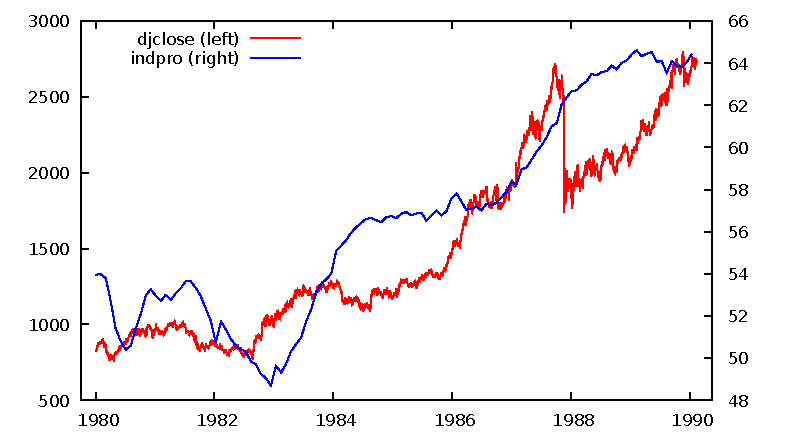
\includegraphics{figures/midas_daily_plot}
  \caption{Monthly industrial production and daily Dow Jones close}
  \label{fig:daily}
\end{figure}

%%% Local Variables:
%%% mode: latex
%%% TeX-master: "gretl-guide"
%%% End:
